\section{Frequenzanalyse}{107}

\subsubsection{Bestimmung Frequenzspektrum pro Signalkategorie}

\begin{tabular}{l c l}
    \textbf{Periodische} Leistungssignale   & \textrightarrow\ & Fourier-Reihe              \\
    Energiesignale                          & \textrightarrow\ & Fourier-Transformation     \\
    Aperiodische Leistungssignale           & \textrightarrow\ & AKF \& Leistungsspektrum 
\end{tabular}


\subsubsection{Periodizität}

Ein periodisches Signal $a(t)$ \textbf{behält} durch Addition oder Subtraktion eines Signals $b(t)$ 
\textbf{gleicher oder vielfacher Periode $\bm{T}$ seine Periodizität} 
$$ c(t + T) = a(t + T) \pm b(t + T) = a(t) \pm b(t) = c(t) $$


\subsubsection{Orthogonalitätsrelationen Trigo-Funktionen}{109}

Die Orthogonalitätsrelationen können bei der Berechnung der Fourier-Reihen hilfreich sein.

\vspace{0.2cm}

\begin{tabular}{ll}
	$\int \limits_{0}^{T} \cos(m \, \omega_f \, t) \cdot \cos(n \, \omega_f \, t) \, \diff t = 
    \begin{cases}
    T,              & m = n = 0 \\
    \frac{T}{2},    & m = n > 0 \\
    0,              & m \neq n
    \end{cases} $ 
    & $(m, \; n \in \mathbb{N}_0)$ \\
    \\
    $\int \limits_{0}^{T} \sin(m \, \omega_f \, t) \cdot \sin(n \, \omega_f \, t) \, \diff t =      		
	\begin{cases}
    \frac{T}{2},    & m = n  \\
    0,              & m \neq n
    \end{cases} $ 
    & $(m, \; n \in \mathbb{N})$ \\
    \\
    $\int \limits_{0}^{T} \cos(m \, \omega_f \, t) \cdot \sin(n \, \omega_f \, t) \, \diff t = 0 $ 	
    & $(m \in \mathbb{N}_0, \; n \in \mathbb{N})$ 
\end{tabular}
	
\vspace{0.2cm}

$$ \sin(\alpha \pm \beta) = \sin(\alpha) \cdot \cos(\beta) \pm \cos(\alpha) \cdot \sin(\beta) $$
	

\subsection{Fourier-Reihe -- Trigonometrische Darstellung}{108}

Ist $f(t)$ eine \textbf{eindeutige}, reelle, stückweise \textbf{monotone} und \textbf{differenzierbare, periodische Funktion} mit der
\textbf{Primitivperiode $T$}, so lässt sich eine \textbf{Fourier-Reihe} von $f(t)$ entwickeln.

$$ \boxed{ f(t) \rightsquigarrow \frac{a_0}{2} + \sum\limits_{k=1}^\infty \Bigg( a_k\, \cos \Big(\frac{2 \, \pi \, k}{T} \, t \Big) + b_k\, \sin \Big(\frac{2 \, \pi \, k}{T} \, t \Big)  \Bigg) } $$

\textbf{$\bm{\frac{a_0}{2}}$ entspricht dem Mittelwert (Gleichstromanteil) der Funktion $\bm{f(t)}$ auf dem Intervall [$\bm{0}$ ; $\bm{T}$)} 


\subsubsection{Berechnung der Fourier-Koeffizienten}
\label{Berechnung der Fourier-Koeffizienten - Trigonometrisch}

$$ a_0 = \frac{2}{T} \cdot \int \limits_{0}^{T} f(t) \, \diff t $$
$$ a_k = \frac{2}{T} \cdot \int \limits_{0}^{T} f(t) \cdot \cos \Big( \frac{2 \, \pi \, k}{T} \, t \Big) \, \diff t \quad \text{ für } k \in N_0 $$
$$ b_k = \frac{2}{T} \cdot \int \limits_{0}^{T} f(t) \cdot \sin \Big( \frac{2 \, \pi \, k}{T} \, t \Big) \, \diff t \quad \text{ für } k \in N $$

\textbf{\crd{ \textrightarrow\ Trigo-Produkte in Integralen in SUMMEN umwandeln!!}}


\subsection{Fourier-Reihe - Harmonische Darstellung}{113}

Statt mit Sinus- und Cosinus-funktionen kann die Fourier-Reihe auch nach Betrag und Phase (Periode $T$) dargestellt werden:

$$  \boxed{ f(t) \rightsquigarrow \frac{a_0}{2} + \sum\limits_{k=1}^\infty \Big( d_k\, \cos \big(\frac{2 \, \pi \, k}{T} \, t + \phi_k \big) \Big) } $$

\begin{minipage}[c]{0.48\columnwidth}
    $$ \text{Betrag:} \quad d_k = \sqrt{a_k^2 + b_k^2} $$
\end{minipage}
\hfill
\begin{minipage}[c]{0.48\columnwidth}
    $$ \text{Phase:} \quad \phi_k = -\arctan \big( \frac{b_k}{a_k} \big) + n \, \pi $$ 
\end{minipage}


\subsubsection{Berechnung der Fourier-Koeffizienten}

\textrightarrow\ Berechnung von $a_k$ und $b_k$ gemäss Abschnitt ~\ref{Berechnung der Fourier-Koeffizienten - Trigonometrisch} \\
\textrightarrow\ Umrechung in Betrag und Phase

	
\subsection{Fourier-Reihe -- Komplexe Darstellung}{114}

Ausgehend von der \textbf{Eulerschen Formeln} kann man die Fourier-Reihe mit \textbf{Exponentialfunktionen} anstelle von Winkelfunktionen formulieren

\vspace{0.2cm}

\begin{minipage}{0.48\columnwidth}
    $$ \sin(t) = \frac{\e^{\jimg t} - \e^{- \jimg t}}{2j} $$ 
\end{minipage}
\hfill
\begin{minipage}{0.48\columnwidth}
    $$ \cos(t) = \frac{\e^{\jimg t} + \e^{- \jimg t}}{2} $$
\end{minipage}

\vspace{0.2cm}

$$  \boxed{ f(t) \rightsquigarrow \sum\limits_{k=-\infty}^\infty c_k \, e^{\jimg \frac{2 \, \pi \, k \, t}{T}} } $$


\subsubsection{Berechnung der komplexen Fourier-Koeffizienten $\bm{c_k}$}

\vspace{-0.2cm}

$$c_k = \overline{c_{-k}} = \frac{1}{T} \int\limits_0^T f(t) \cdot e^{- \jimg \frac{2 \, \pi \, k \, t}{T}}   \, \diff t =
\begin{cases}
\frac{a_0}{2}                       & \text{für } k = 0 \\
\frac{1}{2} (a_k - \jimg \, b_k)        & \text{für } k > 0 \\
\frac{1}{2} (a_{-k} + \jimg \, b_{-k})  & \text{für } k < 0
\end{cases} $$

$$ \text{Es gilt:} \quad a_k = c_k + c_{-k} \text{ und } b_k = \jimg (c_k - c_{-k}) $$ 

		
\subsection{Umrechnung der Fourier-Koeffizienten}

\renewcommand{\arraystretch}{1.5}
\begin{tabular}{ll}
    $c_k = \overline{c_{-k}} = \frac{a_k - \jimg \, b_k }{2}$   & ($k = 0, \, 1, \,  2\, \ldots \, ,$ wobei $b_0 = 0$)  \\
    $a_k = 2 \, \RE(c_k) = c_k + c_{-k}$                        & ($k = 0, \, 1, \,  2\, \ldots$)                       \\
    $b_k = -2 \, \IM(c_k) = \jimg(c_k - c_{-k})$                & ($k = 1, \,  2\, \ldots$)                             \\
    $d_k = 2 \, |c_k| = \sqrt{a_k^2 + b_k^2}$                   & $\phi_k = - \arctan \Big( \frac{b_k}{a_k} \Big)$
\end{tabular}
\renewcommand{\arraystretch}{1}
		
		
\subsection{Tipps zur Berechnung der Koeffizienten}{115}

\subsubsection{Achsensymmetrien}

\begin{center}
    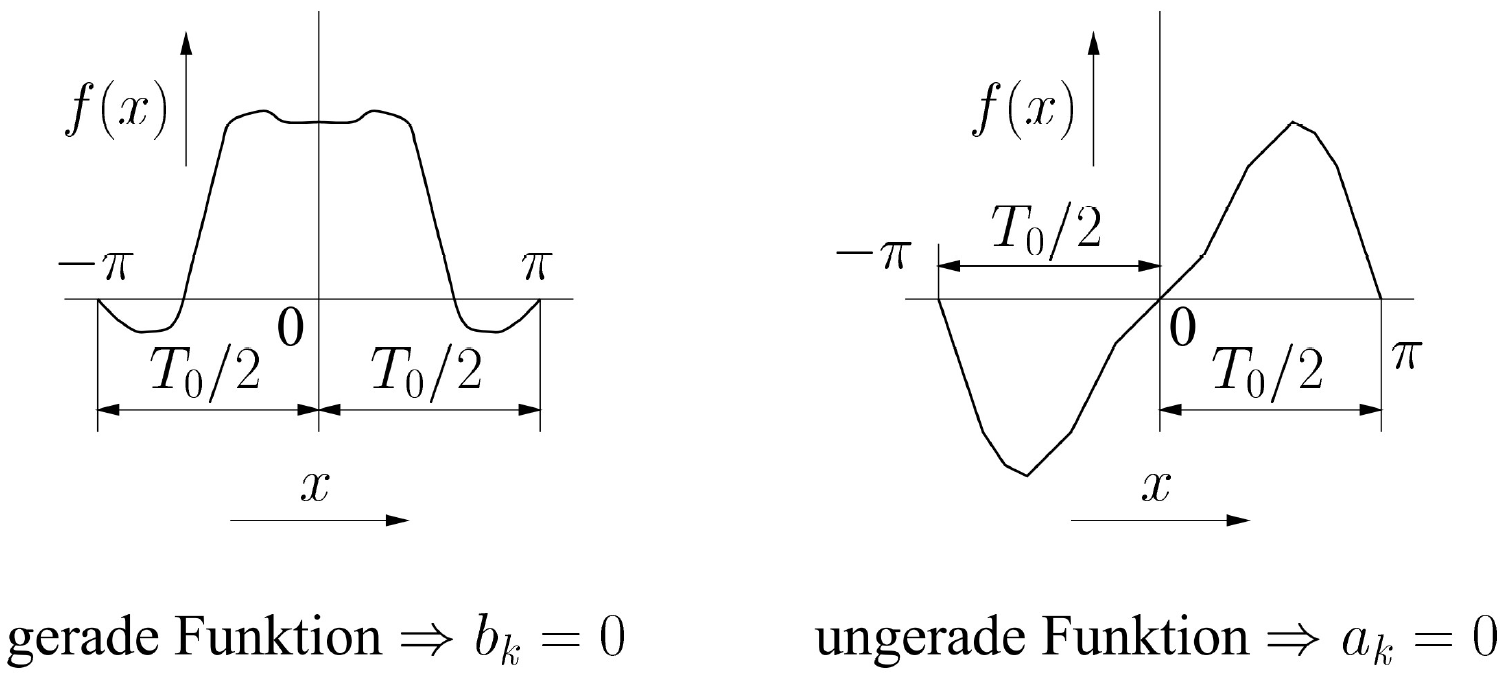
\includegraphics[width=0.75\columnwidth]{images/achsensymmetrie.png}

    \vspace{0.2cm}

    \begin{tabular}{lll}
        $f(t)$ gerade   & $a_k = \frac{4}{T} \cdot \int \limits_{0}^{\frac{T}{2}} f(t) \cdot \cos \Big( \frac{2 \pi k}{T} t \Big) \, \diff t$   & $b_k = 0$ \\
        \\
        $f(t)$ ungerade & $b_k = \frac{4}{T} \cdot \int \limits_{0}^{\frac{T}{2}} f(t) \cdot \sin \Big( \frac{2 \pi k}{T}  t \Big) \, \diff t$  & $a_k = 0$
    \end{tabular}
\end{center}	
		
\subsubsection{Symmetrie der Halbperioden}

Haben die Halbperioden die \textbf{gleiche Form} und sind in der \textbf{gleichen Lage zur x-Achse}, also $f(x) = f(x + \pi)$,
so gibt es nur Glieder mit \textbf{geraden Argumenten}.

\vspace{0.2cm}	

Ist aber nur die \textbf{Form gleich} und die \textbf{Lage zur $\bm{x}$-Achse verschieden}, also $f(x) = - f(x + \pi)$, so gibt es 
nur Glieder mit \textbf{ungeraden Argumenten}.

\begin{center}
    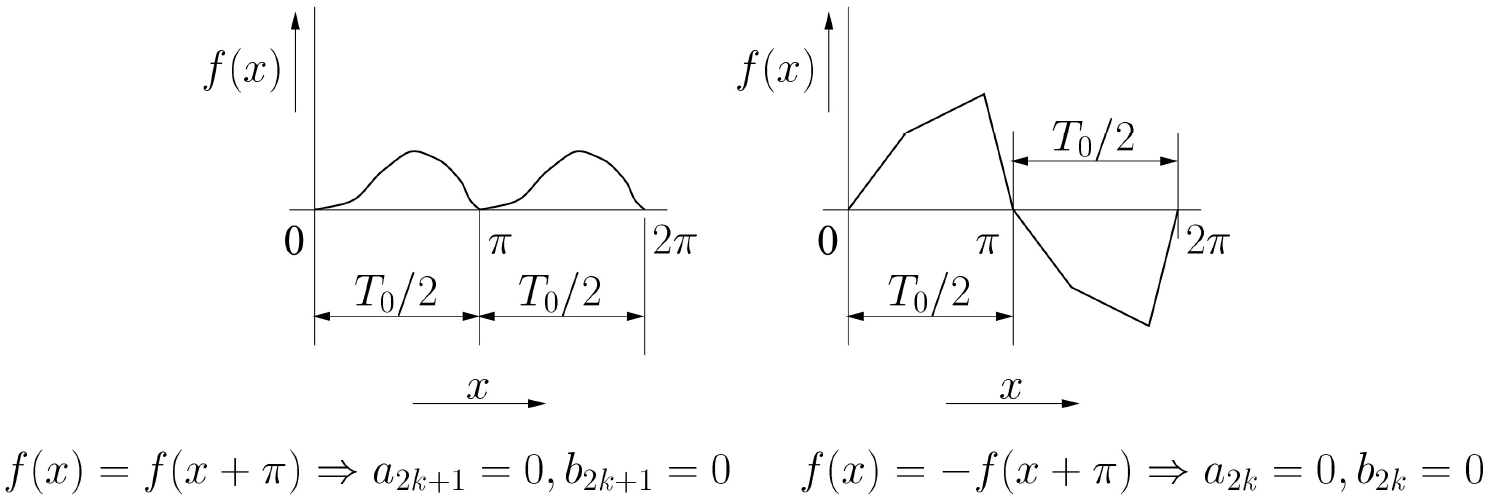
\includegraphics[width=0.9\columnwidth]{images/symmetrie_halbperioden.png}

    \vspace{0.2cm}

    \begin{tabular}{llll}
        links   & $a_{2k+1} = 0$    & $b_{2k+1} = 0$    & $a_0 \neq 0$ \\
        rechts  & $a_{2k} = 0$      & $b_{2k} = 0$      & $a_0 = 0$
    \end{tabular}
\end{center}


\subsection{Fourier-Koeffizienten und Leistung}{119}

Für den quadratischen Mittelwert $X^2$, also für die \textbf{Leistung} einer periodischen Funktion $x(t)$ gilt:

$$ \boxed{ X^2 = \sum\limits_{k=-\infty}^{\infty} |c_k|^2 = |c_0|^2 + 2 \, \sum\limits_{k=1}^{\infty} |c_k|^2 
    = \Big( \frac{a_0}{2} \Big)^2 + \sum\limits_{k=1}^{\infty} \frac{a_k^2 + b_k^2}{2} 
    = \Big( \frac{a_0}{2} \Big)^2 + \sum\limits_{k=1}^{\infty} \frac{d_k^2}{2} } $$		
		
		
\subsection{Gibbs'sches Phänomen}{112}

\begin{minipage}{0.35\columnwidth}
    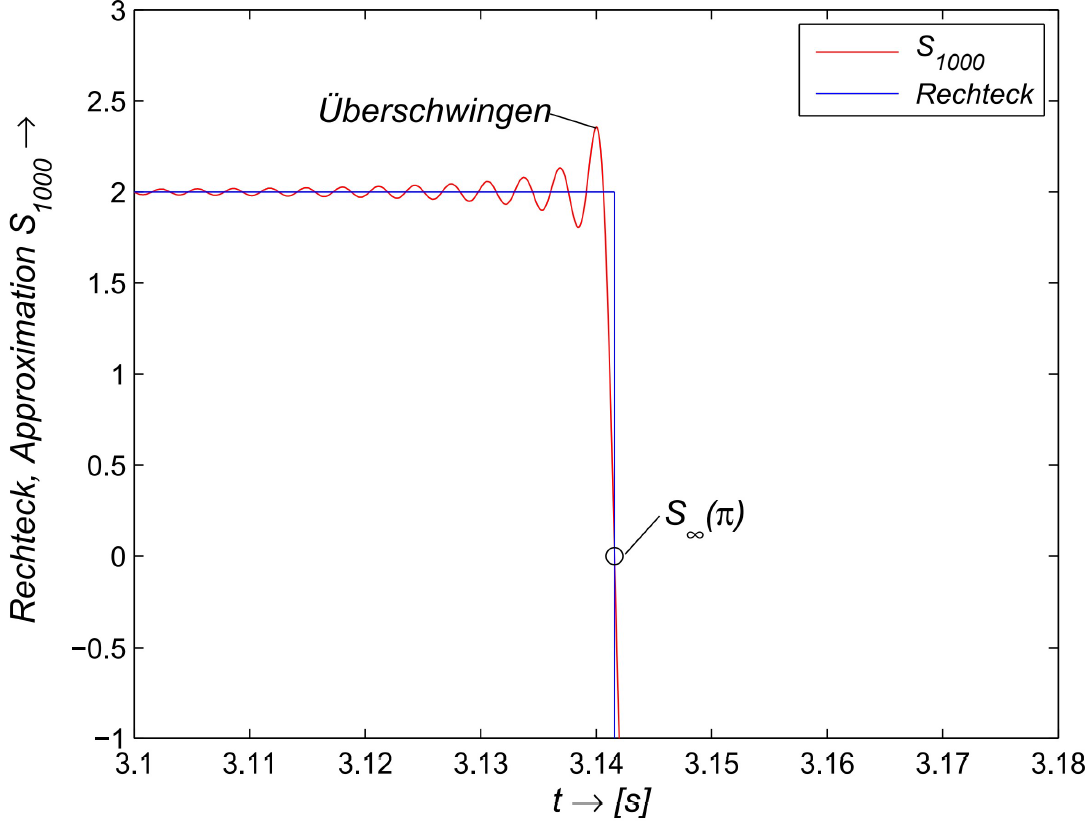
\includegraphics[width=\columnwidth]{images/gibbssches_phaenomen.png}
\end{minipage}
\hfill
\begin{minipage}{0.64\columnwidth}
    \raggedright
    An \textbf{Unstetigkeitsstellen} entsteht immer ein \textbf{Überschwingen}

    \vspace{0.2cm}

    \begin{itemize}
        \item ca. 18 \% der Amplitude ('peak')
        \item ca. 9 \% der Sprunghöhe ('peak-peak')
    \end{itemize}
\end{minipage}

\vspace{0.2cm}

Wenn $f(t)$ an der Stelle $t = t_0$ eine \textbf{Unstetigkeit} besitzt, dann ist die \textbf{Approximation} $S_{\infty}$ der 
Funktion $f(t)$ nicht nahe am richtigen Wert $f(t)$, egal wieviele Sinus- und Cosinus-Funktionen man verwendet.

$$ S_{\infty} = \frac{f(x_0^+) + f(x_0^-)}{2}  \quad \text{Mitte der Sprungstelle} $$

\columnbreak

